\chapter{Preliminares}

\section{Estado del arte}

Cada día se producen grandes avances en muchos campos con el uso de inteligencia artificial, sin embargo, su uso en el campo de la composición musical no está muy explotado. A pesar de esto si existen algunas herramientas que podemos usar como referencias para el desarrollo de nuestro trabajo.

\subsection{Música adaptativa para videojuegos}

% Hablar de Brian Eno y la música generativa. Introducir FMOD como herramienta para música adaptativa en los videojuegos.
%Mencionar las dos posibles alternativas de generar música, es decir, de forma simbólica y luego añadir los instrumentos, o de forma directa. Decir que nos decantamos por la simbólica, pra introducir la siguiente subsección
Debido a que en un videojuego no podemos saber cuanto tiempo permanecerá el jugador en una zona, ni en qué instante de tiempo realizará acciones que podríamos destacar usando la música, la forma tradicional de hacer música no funciona en los videojuegos. Es aquí donde entra la música adaptativa.

La música adaptativa consiste en componer música de forma que esta se acomode a lo que esté sucediendo en el videojuego. Para esto se utilizan distintas técnicas que se diferencian de la composición tradicional. Hay 2 maneras principales de componer música adaptativa:
\begin{itemize}
    \item Composición horizontal: consiste en componer una canción formada por varias secciones y realizar saltos temporales entre dichas secciones. Este tipo de composición se acerca más a la tradicional, teniendo como peculiaridad que las secciones deben de funcionar por separado y poder ciclarse. 
    \item Composición vertical: en esta, se utilizan diferentes capas que se activan o desactivan para crear diferentes secciones. Estas capas pueden incluir: melodía, armonía, línea de bajo, base rítmica, ambientes, etc. En este trabajo se generarán diferentes capas para utilizar este tipo de composición.
\end{itemize}

\subsubsection{FMOD}

FMOD es un motor de efectos de sonido para videojuegos y aplicaciones desarrollado por Firelight Technologies, el cual consiste principalmente en una API de código. Se utiliza para sonorizar videojuegos y además, puede usarse para crear música adaptativa.

Posee una aplicación de escritorio llamada \textit{FMOD Studio}, la cual permite tener una interfaz gráfica para realizar la mayor parte de las acciones que se pueden realizar utilizando la API de código.

Con FMOD podemos crear variables configurables desde el propio juego, para controlar aspectos como qué parte de la canción suena, volumen, intensidad de la música, etc. Además, presenta la posibilidad de no usar una \textit{timeline}, para crear composiciones \textit{no lineales}, es decir, música que no tiene una estructura fija, sino que depende de la configuración de las variables en un momento dado.

\subsection{Música generativa}
La música generativa es un tipo de música el cual se va creando y evolucionando a medida que se va reproduciendo, de forma que cambia cada vez que suena. Uno de los mayores exponentes de esta corriente musical es Brian Eno, un artista enfocado principalmente a la composición de música \textit{ambient}. En el trabajo de Eno podemos apreciar composiciones que utilizaban software de sintetizadores para introducir partes que se reproducen o no de manera aleatoria para crear una canción única para cada vez que se reproducen.

Este tipo de música se puede aplicar a videojuegos, y, aunque no representa el grueso de nuestro trabajo, es una inspiración a la hora de plantear la composición de las distintas partes de nuestras canciones.

\subsection{Generación de música como audio}
La generación de audio es un campo con muchos avances en los últimos años. Especialmente el último año, ha sufrido una mejora tan grande que ha pasado a ser la opción predilecta para los usuarios. Normalmente, este tipo de modelos se basan en introducir \textit{prompts} para generar una canción del estilo que se quiera.

Esta generación tiene como ventaja el gran acceso a información disponible, ya que hay más \textit{datasets} de música ya renderizada que de música simbólica. Por este motivo últimamente se ha visto que puede generar canciones que pueden pasar por canciones compuestas por una persona.

Sin embargo, este método no proporciona mucha flexibilidad a la hora de poder variar secciones de la composición y, por lo tanto, no se utiliza en este trabajo. Aunque podría ser una opción más a explorar para generar secciones de música adaptativa.

\subsection{Generación de música simbólica}

    \subsubsection{Generación con Cadenas de Markov}
    En el paper de \citet{MarkovChainPaper}, se detalla cómo utilizar cadenas de Markov para la generación de fragmentos musicales con el estilo de un compositor específico.

    En este, se centran en los aspectos matemáticos del modelo de Markov, no tanto en la calidad musical de la generación, que resulta más como una prueba que como una composición seria. Sin embargo, el tratamiento simbólico de la música en dicho paper resulta interesante y se ha utilizado como apoyo para desarrollar nuestros modelos de generación.

    \subsubsection{Magenta} 
    \label{subsec:definicionMagenta}

    Magenta es un proyecto de investigación propiedad de Google, compuesto por varios modelos de \textit{machine learning}. Estos modelos están entrenados para generar tanto música como dibujos.

    Particularmente, los modelos entrenados con música pueden realizar varias funcionalidades. Existen modelos que generan melodías, modelos que continúan una melodía dada, generar baterías, \textit{autoencoders} que permiten humanizar baterías, armonizar una melodía dada... Podemos encontrar estos modelos y más en el repositorio de Magenta \citep{MagentaRepo} o en su web \citep{MagentaWeb}.

    Magenta contiene además un plugin para la DAW Ableton llamado Magenta Studio \citep{MagentaStudio}. Dicho plugin fue además porteado a aplicación de escritorio para Windows. En este plugin encontramos varios programas que desmuestran la funcionalidad de Magenta: 
    \begin{itemize}
        \item Generate, que genera melodías de 4 compases.
        \item Continue, que continúa una melodía de entrada un número N de compases.
        \item Drumify, que crea una base de batería dado un ritmo de input.
        \item Interpolate, que crea una melodía o base de tambor combinando 2 de entrada.
        \item Groove, que humaniza una base de tambor para que suene como una persona.
    \end{itemize}


\section{Pequeña introducción a la música}\label{sec:arm:armonia}

\label{arm:notas_musicales}
Nos centraremos en la notación musical occidental, utilizada prácticamente en todas las canciones que escuchamos diariamente, en la que los sonidos se dividen en conjuntos de 12 notas musicales, cada una con un nombre diferente, definiendo nota musical como un símbolo que representa una frecuencia determinada. Para entender de dónde viene esta división utilizaremos como base la nota A4 (La4), con una frecuencia de 440Hz y duplicaremos su frecuencia a 880Hz, obteniendo así A5 (La5). Estas dos notas comparten nombre, ya que si las escucháramos nos sonarían muy familiares entre sí. Esto tiene una explicación física: al reproducir esa frecuencia (frotando una cuerda, elevando una columna de aire...), no solo se genera la frecuencia fundamental, sino que también se producen armónicos, que son múltiplos enteros de la frecuencia fundamental. Se llama octava a la distancia que separa una frecuencia de su duplicación, esto explica ahora los número escritos al lado de cada nota musical: A3 = 220Hz, A4 = 440Hz, A5 = 880Hz. Sabiendo esto se decidió entonces dividir la octava en 12 notas musicales, perceptualmente equidistantes. Es la llamada afinación temperada. Sacamos como conclusión que el conjunto de sonidos utilizados está comprendido por las 12 notas musicales, cada una pudiéndose encontrar en una octava distinta. 

Entrando en otra capa de profundidad, en la música se pueden encontrar diversos elementos si nos fijamos en las notas que conforman una canción, como por ejemplo el ritmo, sin embargo, en los dos en los que se quiere hacer hincapié ahora son:
\begin{enumerate}
    \item[\textbullet] \textbf{Melodía}: evolución horizontal de las notas a lo largo de una canción. Es la parte más reconocible de esta. En una composición musical es la parte que generalmente se canta o se toca de manera prominente. 
    \item[\textbullet] \textbf{Armonía}: asociaciones verticales de las notas. La armonía proporciona un acompañamiento sonoro a la melodía principal y contribuye a enriquecer la textura musical. 
\end{enumerate}

\section{Pequeña introducción a la armonía}

Como se acaba de explicar, la armonía se refiere a la combinación simultánea de notas musicales que suenan de manera agradable y coherente entre sí. Para entender tanto la armonía, como los algoritmos que se quieren mostrar en futuros apartados del TFG, es necesario interiorizar los siguientes conceptos, que se intentarán explicar de la manera más resumida posible. Cabe recalcar que la explicación se realiza en el contexto de la armonía moderna, la cual difiere en algunos puntos de la clásica. Sin embargo, al tratarse de una introducción, la mayoría de conceptos que van a ser mostrados se comparten entre ambas doctrinas. A pesar de ello, una de las primeras cosas en las que sí difieren es en el nombre de las notas. A partir de ahora se utilizará el cifrado americano: (Figura \ref{tab:cifrado_americano})

\begin{table}[h]
    \centering
    \begin{tabular}{c||c|c|c|c|c|c|c}
        \textbf{Nota} & Do & Re & Mi & Fa & Sol & La & Si \\
        \hline
        \textbf{Cifrado} & C & D & E & F & G & A & B \\
    \end{tabular}
    \caption{Cifrado americano}
    \label{tab:cifrado_americano}
\end{table}    

\subsection{Intervalos}\label{sec:arm:intervalos}

\begin{figure}[h]
    \centering
    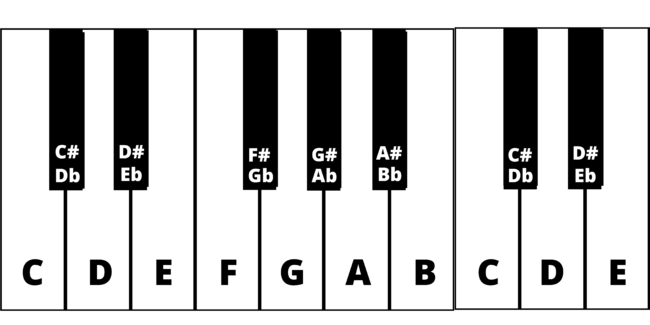
\includegraphics[width = 0.5\textwidth]{Imagenes/Bitmap/piano.png}
    \caption{Notas en el piano}
    \label{fig:pianoImage}
\end{figure}

Un intervalo es la distancia que existe entre dos notas. Un semitono es la distancia mínima que puede existir entre dos notas. Un tono es igual a dos semitonos. Por ejemplo, en la Figura \ref{fig:pianoImage} se observa que la distancia entre el primer C y el primer E es de 4 semitonos (las teclas negras también cuentan como notas musicales aunque tengan nombres un poco especiales). Entre C y C\# o entre E y F, por ejemplo, hay un semitono. Dependiendo del número de semitonos que tenga un intervalo, este tendrá un nombre y simbología diferente: (Tabla \ref{tab:tabla_intervalos})

\begin{table}[H]
    \centering
    \begin{tabular}{c|c|c}
        \textbf{Símbolo} & \textbf{Nombre} & \textbf{Nº Semitonos} \\
        \hline
        1 (T) & Tónica & 0 \\
        b2 & Segunda menor & 1 \\
        2 & Segunda mayor & 2 \\
        b3 & Tercera menor & 3 \\
        3 & Tercera mayor & 4 \\
        4 & Cuarta justa & 5 \\
        \#4 & Cuarta aumentada & 6 \\
        5b & Quinta disminuida & 6 \\
        5 & Quinta justa & 7 \\
        b6 & Sexta menor & 8 \\
        6 & Sexta mayor & 9 \\
        b7 & Séptima menor & 10 \\
        7 & Séptima mayor & 11 \\
        8 & Octava & 12 \\
    \end{tabular}
    \caption{Tabla de intervalos}
    \label{tab:tabla_intervalos}
\end{table}

Al observar la Tabla \ref{tab:tabla_intervalos} se puede deducir por contexto que el símbolo 'b' (bemol) reduce en uno el número de semitonos del grado original, así como el símbolo '\#' (sostenido) los aumenta en uno. Por ejemplo, \#6 sería equivalente a una séptima menor (b7), con 10 semitonos ambos.

Con la información de esta tabla, ya podríamos entender afirmaciones tales como 'la quinta justa de C es G' o 'la tercera mayor de B es D\#', por ejemplo, si nos ponemos a contar los semitonos más detenidamente (piano de referencia en la Figura \ref{fig:pianoImage}).

Cabe recalcar que, evidentemente, existen intervalos que se salen de la octava, con más de 12 semitonos. Algunos no muy lejanos tienen incluso nombre propio, por ejemplo, una novena mayor (9), de 14 semitonos. A pesar de ello, lo que se hará en estos casos es interpretar ese intervalo como su relativo si la nota estuviese en el 'mismo rango' que la tónica (nota desde la cual se mide el intervalo). Así, una novena mayor sería equivalente a una segunda mayor, de 2 semitonos y un intervalo de 42 semitonos será interpretado como una quinta disminuida (42 mod 12 = 6 semitonos), por ejemplo. De hecho, siguiendo esta definición, el propio intervalo de octava es redundante, ya que esta es equivalente a la tónica y cumple la misma función (12 mod 12 = 0 semitonos). Por ejemplo, la octava de C4 es C5. Por ello, el intervalo de octava también se debería quitar de la lista.

\subsection{Escalas}\label{sec:arm:escalas}

Se define escala como una secuencia de intervalos ascendentes entre los 12 previos a la octava cuyo primero es siempre la tónica. Tradicionalmente, la mayoría de escalas están formadas por 7 notas o intervalos, las más utilizadas en la música que escuchamos hoy en día son la mayor y la menor: (Tabla \ref{tab:escalas})

\begin{table}[h]
    \centering
    \begin{tabular}{c|c|c|c|c|c|c|c}
        \textbf{Escala mayor} & 1 (T) & 2 & 3 & 4 & 5 & 6 & 7 \\
        \hline
        \hline
        \textbf{Escala menor} & 1 (T) & 2 & b3 & 4 & 5 & b6 & b7 \\
    \end{tabular}
    \caption{Escalas mayor y menor}
    \label{tab:escalas}
\end{table}

Este conjunto de intervalos representa una especie de esqueleto, un molde con el cual se puede crear una sucesión de notas musicales si se establece como tónica cualquiera de las 12 existentes. Cuando se crea una sucesión de grados respecto a una tónica utilizando cualquiera de estas dos escalas, mayor o menor, se estaría hablando de tonalidad. Un grado es la numeración de una nota dentro de la escala a la que pertenece y se escribe en números romanos. Aquí unos cuantos ejemplos de tonalidades mayores y menores (Tablas \ref{tab:tonalidades_mayores} y \ref{tab:tonalidades_menores} respectivamente)

\begin{table}[h]
    \centering
    \begin{tabular}{c|c|c|c|c|c|c|c}
     & \textbf{I}& \textbf{II} & \textbf{III} & \textbf{IV} & \textbf{V} & \textbf{VI} & \textbf{VII} \\
        \hline
        \hline
        \textbf{C mayor} & C & D & E & F & G & A & B \\
        \hline
        \textbf{D mayor} & D & E & F\# & G & A & B & C\# \\
        \hline
        \textbf{Bb mayor} & Bb & C & D & Eb & F & G & A \\
    \end{tabular}
    \caption{Tonalidades mayores}
    \label{tab:tonalidades_mayores}
\end{table}

\begin{table}[h]
    \centering
    \begin{tabular}{c|c|c|c|c|c|c|c}
        & \textbf{I} & \textbf{II} & \textbf{bIII} & \textbf{IV} & \textbf{V} & \textbf{bVI} & \textbf{bVII} \\
        \hline
        \hline
        \textbf{C menor} & C & D & Eb & F & G & Ab & Bb \\
        \hline
        \textbf{D menor} & D & E & F & G & A & Bb & C \\
        \hline
        \textbf{Bb menor} & Bb & C & Db & Eb & F & Gb & Ab \\
    \end{tabular}
    \caption{Tonalidades menores}
    \label{tab:tonalidades_menores}
\end{table}

A parte de estas dos escalas, existen muchas otras más que se utilizan regularmente a la hora de componer música. Algunos ejemplos: (Tabla \ref{tab:otras_escalas})

\begin{table}[H]
    \centering
    \begin{tabular}{c|c|c|c|c|c|c|c}       
        \textbf{Pentatónica mayor} & 1 (T) & 2 & 3 & 5 & \multicolumn{1}{c}{6} \\
        \hline
        \textbf{Pentatónica menor} & 1 (T) & b3 & 4 & 5 & \multicolumn{1}{c}{b6} \\
        \hline
        \textbf{Hexatónica} & 1 (T) & 2 & 3 & \#4 & \#5 & \multicolumn{1}{c}{\#6}  \\
        \hline
        \textbf{Menor armónica} & 1 (T) & 2 & b3 & 4 & 5 & b6 & 7 \\ 
        \hline
        \textbf{Frigia} & 1 (T) & b2 & b3 & 4 & 5 & b6 & b7 \\
        \hline
        \textbf{Mixolidia} & 1 (T) & 2 & 3 & 4 & 5 & 6 & b7 \\             
    \end{tabular}
    \caption{Otras escalas}
    \label{tab:otras_escalas}
\end{table}

\subsection{Acordes}\label{sec:arm:acordes}

Aunque no todo el mundo estaría de acuerdo con esta definición, vamos a decir que un acorde es un conjunto de dos o más notas tocadas de forma simultánea. La definición es en cierta medida similar a la de una escala, ya que un acorde no deja de ser un conjunto de intervalos ascendentes, en el que el primero es siempre la tónica del acorde. También se cumple esa propiedad de 'molde' a la hora de establecer una nota musical como tónica del acorde. Los acordes más comunes están formados por tres notas (tríadas) y dependiendo del conjunto de intervalos se pueden conseguir diferentes sonoridades: (Tablas \ref{tab:triads} y \ref{tab:triadsC})

\begin{table}[h]
    \centering
    \begin{tabular}{c|c|c|c|c}       
        \textbf{Nombre} & \textbf{Símbolo} & \multicolumn{3}{c}{\textbf{Intervalos}} \\
        \hline
        \hline
        \textbf{Acorde mayor} & & 1 (T) & 3 & 5 \\
        \hline
        \textbf{Acorde menor} & - & 1 (T) & b3 & 5 \\
        \hline
        \textbf{Acorde aumentado} & + & 1 (T) & 3 & \#5 \\
        \hline
        \textbf{Acorde disminuido} & -b5 & 1 (T) & b3 & b5 \\
    \end{tabular}
    \caption{Tríadas}
    \label{tab:triads}
\end{table}

\begin{table}[h]
    \centering
    \begin{tabular}{c|c|c|c|c}       
        \textbf{Nombre} & \textbf{Símbolo} & \multicolumn{3}{c}{\textbf{Notas}} \\
        \hline
        \hline
        \textbf{C mayor} & C & C (T) & E & G \\
        \hline
        \textbf{C menor} & C- & C (T) & Eb & G \\
        \hline
        \textbf{C aumentado} & C+ & C (T) & E & G\# \\
        \hline
        \textbf{C disminuido} & C-b5 & C (T) & Eb & Gb \\
    \end{tabular}
    \caption{Tríadas en C}
    \label{tab:triadsC}
\end{table}

\label{arm:armonia_escala}
Se define como armonía de una escala el conjunto de acordes que se pueden formar utilizando únicamente las notas (o intervalos) de la escala. Esto puede chocar con la definición de acorde, ya que, como tal, puede haber miles de tipos de acordes diferentes si atendemos a toda la combinatoria, así que, por ahora, solo tendremos en cuenta los tipos de acordes definidos en la Tabla \ref{tab:triads}. Este concepto es más difícil de deducir y explicar, así que recomiendo la visualización de este\footnote{\url{https://www.youtube.com/watch?v=dMwVB3BWcjI}} vídeo en el que el autor encuentra la armonía de la escala C mayor y pasa el resultado a grados, además de repasar otros conceptos vistos por encima anteriormente. Se obtiene el siguiente resultado: (Tabla \ref{tab:grados_C})

\begin{table}[h]
    \centering
    \begin{tabular}{c|c||c|c}
        \textbf{Grado} & \textbf{Acorde} & \textbf{Nota} & \textbf{Acorde} \\
        \hline
        I &  & C & C \\
        II & - & D & D- \\
        III & - & E & E- \\
        IV &  & F & F \\
        V &  & G & G \\
        VI & - & A & A- \\
        VII & -b5 & B & B-b5 \\
    \end{tabular}
    \caption{Escala mayor en grados y en C}
    \label{tab:grados_C}
\end{table}

Como se puede observar, en la escala mayor se forma una tríada mayor a partir de los grados 1, 4 y 5, una menor a partir de los grados 2, 3 y 6, una disminuida a partir del grado 7 y no existe ningún grado del cual se forme una tríada aumentada. Esto significa que sea cual sea la tónica de una escala, en este caso, la escala mayor, los acordes correspondientes a cada grado serán siempre del mismo tipo. Por lo tanto, si se quiere deducir la armonía de una escala diferente, por ejemplo, la escala menor, los acordes correspondientes a cada grado serán distintos a los de la escala mayor, pero serán del mismo tipo si se varía la tónica. Además, el hecho de que solo se forme un acorde por cada grado es debido a una particularidad propia de la escala mayor y a que hemos escogido un número muy reducido de acordes. Vamos a tener en cuenta ahora el siguiente grupo de acordes de cuatro notas (cuatríadas), que se sumarán al anterior grupo: (Tabla \ref{tab:cuatriads})

\begin{table}[h]
    \centering
    \begin{tabular}{c|c|c|c|c|c}       
        \textbf{Nombre} & \textbf{Símbolo} & \multicolumn{4}{c}{\textbf{Intervalos}} \\
        \hline
        \hline
        \textbf{Acorde mayor con séptima} & maj7 & 1 (T) & 3 & 5 & 7\\
        \hline
        \textbf{Acorde menor con séptima} & -7 & 1 (T) & b3 & 5 & b7 \\
        \hline
        \textbf{Acorde de dominante} & 7 & 1 (T) & 3 & 5 & b7\\
        \hline
        \textbf{Acorde semidisminuido} & -7b5 & 1 (T) & b3 & b5 & b7 \\
    \end{tabular}
    \caption{Cuatríadas}
    \label{tab:cuatriads}
\end{table}

A continuación un par de ejemplos que evidencian el anterior párrafo: (Tabla \ref{tab:comparativa_scalas}) 

\begin{table}[h]
    \centering
    \begin{tabular}{c|c|c||c|c|c||c|c|c}
        \multicolumn{3}{c}{} & \multicolumn{3}{c}{\textbf{Escala mayor}}  \\
        \hline  
        \multicolumn{1}{c|}{\textbf{Grados}} & \multicolumn{2}{c||}{\textbf{Acordes}} & \multicolumn{1}{c|}{\textbf{Notas}} & \multicolumn{2}{c||}{\textbf{Acordes}} & \multicolumn{1}{c|}{\textbf{Notas}} & \multicolumn{2}{c}{\textbf{Acordes}} \\
           \hline
    I &     & maj7 & C & C    & Cmaj7 & D   & D      & Dmaj7   \\
        II & -   & -7   &    D  & D-   & D-7   &    E    & E-     & E-7     \\
        III & -   & -7   &    E  & E-   & E-7   &    F\#  & F\#-   & F\#-7   \\
        IV &     & maj7 &    F  & F    & Fmaj7 &    G    & G      & Gmaj7   \\
        V &     & 7    &    G  & G    & G7    &    A    & A      & A7      \\
        VI & -   & -7   &    A  & A-   & A-7   &    B    & B-     & B-7     \\
        VII & -b5 & -7b5 &    B  & B-b5 & B-7b5 &    C\#  & C\#-b5 & C\#-7b5 \\
        \hline
        \multicolumn{3}{c}{} & \multicolumn{3}{c}{\textbf{Escala menor}}  \\
        \hline  
        \multicolumn{1}{c|}{\textbf{Grados}} & \multicolumn{2}{c||}{\textbf{Acordes}} & \multicolumn{1}{c|}{\textbf{Notas}} & \multicolumn{2}{c||}{\textbf{Acordes}} & \multicolumn{1}{c|}{\textbf{Notas}} & \multicolumn{2}{c}{\textbf{Acordes}} \\
           \hline 
    I  & -   & -7   & C  & C-    & C-7    & D & D-   & D-7    \\
        II  & -b5 & -7b5 &    D   & Db-b5 & Db-7b5 &    E  & E-b5 & E-7b5  \\
        bIII &     & maj7 &    Eb  & E     & Emaj7  &    F  & F    & Fmaj7  \\
        IV  & -   & -7   &    F   & F-    & F-7    &    G  & G-   & G-7    \\
        V  & -   & -7   &    G   & G-    & G-7    &    A  & A-   & A-7    \\
        bVI &     & maj7 &    Ab  & Ab    & Abmaj7 &    Bb & Bb   & Bbmaj7 \\
        bVII &     & 7    &    Bb  & Bb    & Bb7    &    C  & C    & C7     \\

    \end{tabular}
    \caption{Comparativa entre escalas (mayor y menor) y tónicas (C y D)}
    \label{tab:comparativa_scalas}
\end{table}

\subsubsection{Inversiones}\label{subsec:inversiones}

\definecolor{rojo}{RGB}{255,0,0} % Rojo
\definecolor{azul}{RGB}{0,0,255} % Azul
\definecolor{verde}{RGB}{0,255,0} % Verde

Un acorde en su estado fundamental es la forma más básica en la que se puede representar dicho acorde. Es el resultado de plasmar en el 'molde' del acorde (Tabla \ref{tab:triads}) la tónica del acorde deseada, por ejemplo C, como se mostró anteriormente en la Tabla \ref{tab:triadsC}. En la Figura \ref{fig:fundamental} se muestra un ejemplo con el acorde de C (Do mayor), conformado por las notas \textcolor{rojo}{C}, \textcolor{verde}{E} y \textcolor{azul}{G}.

\begin{figure}[h]
    \centering
    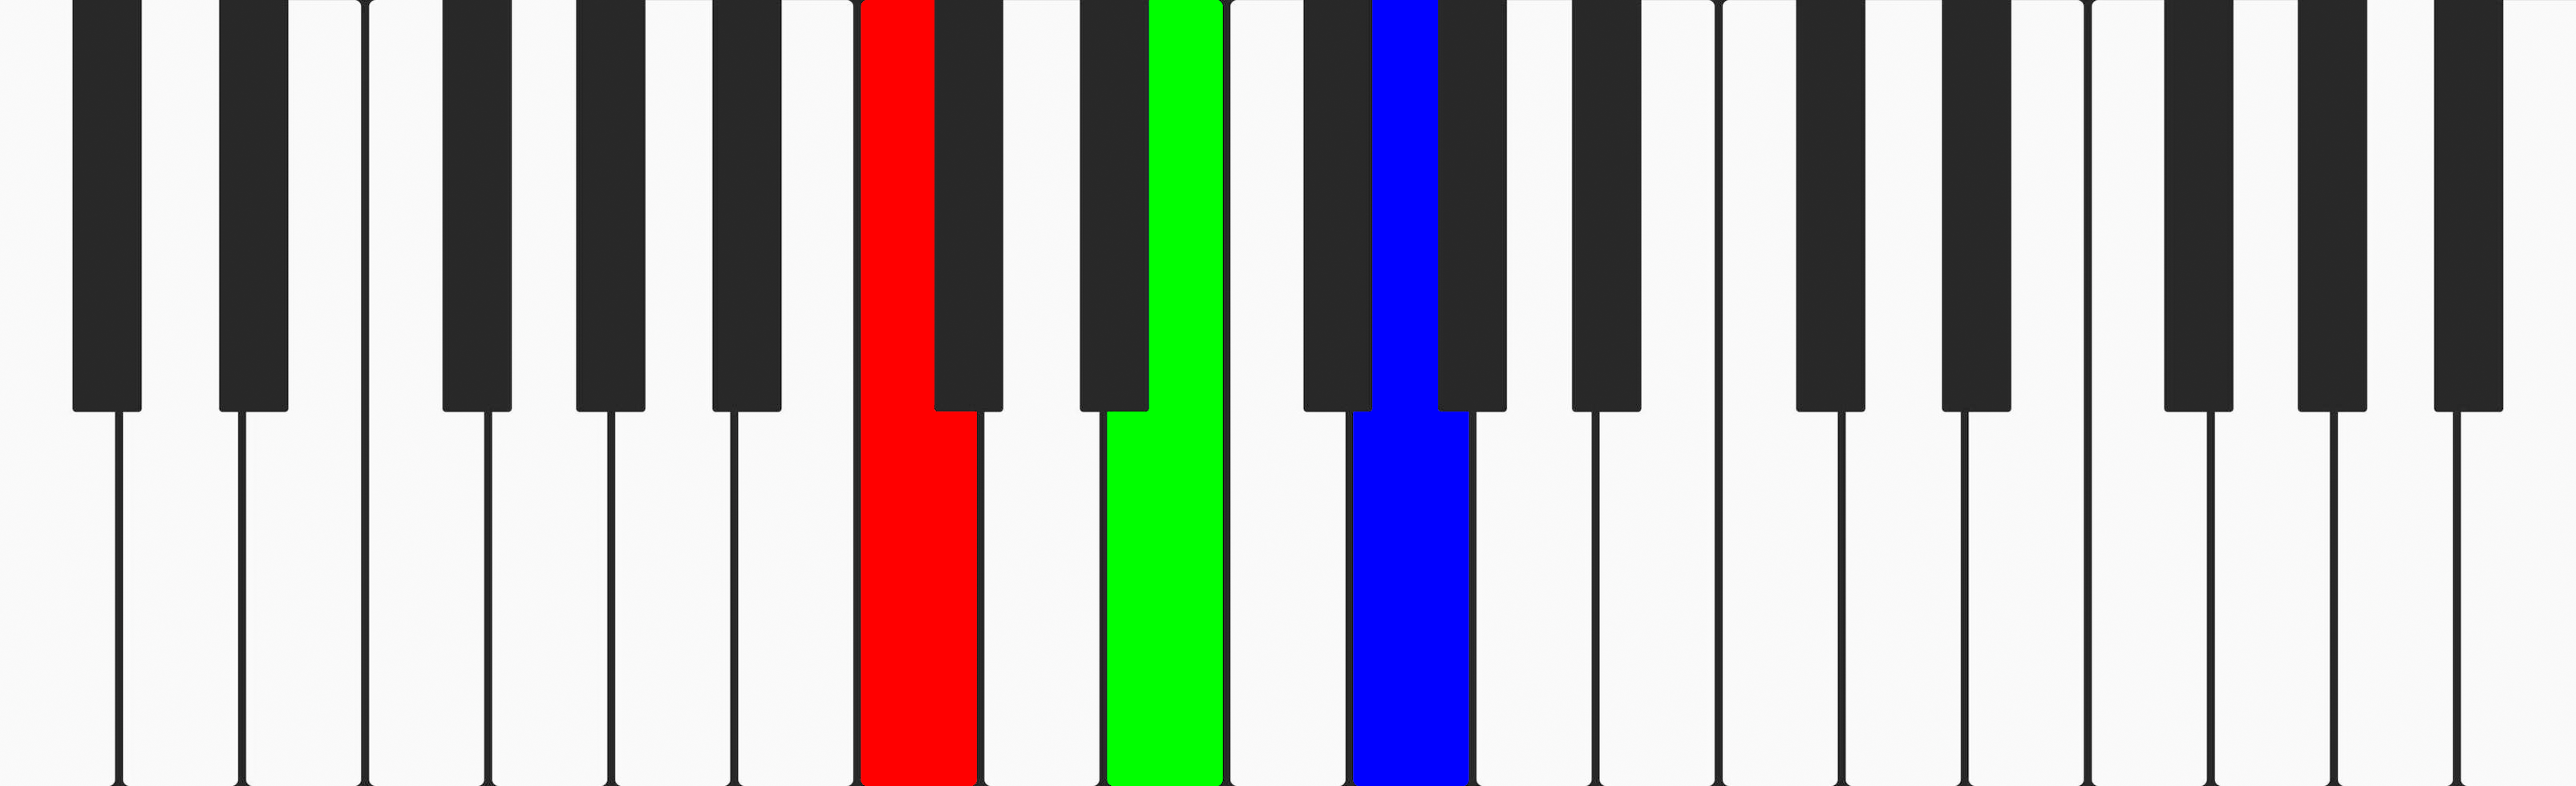
\includegraphics[width = 0.5\textwidth]{Imagenes/Bitmap/fundamental.png}
    \caption{Acorde de C en su estado fundamental}
    \label{fig:fundamental}
\end{figure}

Una inversión consiste en la reordenación de las notas del acorde de forma que la nota mas grave no es la tónica del mismo. Por ejemplo, en una triada la nota más grave también puede ser la segunda o tercera nota del acorde, que corresponderían a la 1º y 2º inversión: (Figuras \ref{fig:inversion1} y \ref{fig:inversion2} respectivamente)

\begin{figure}[h]
    \centering
    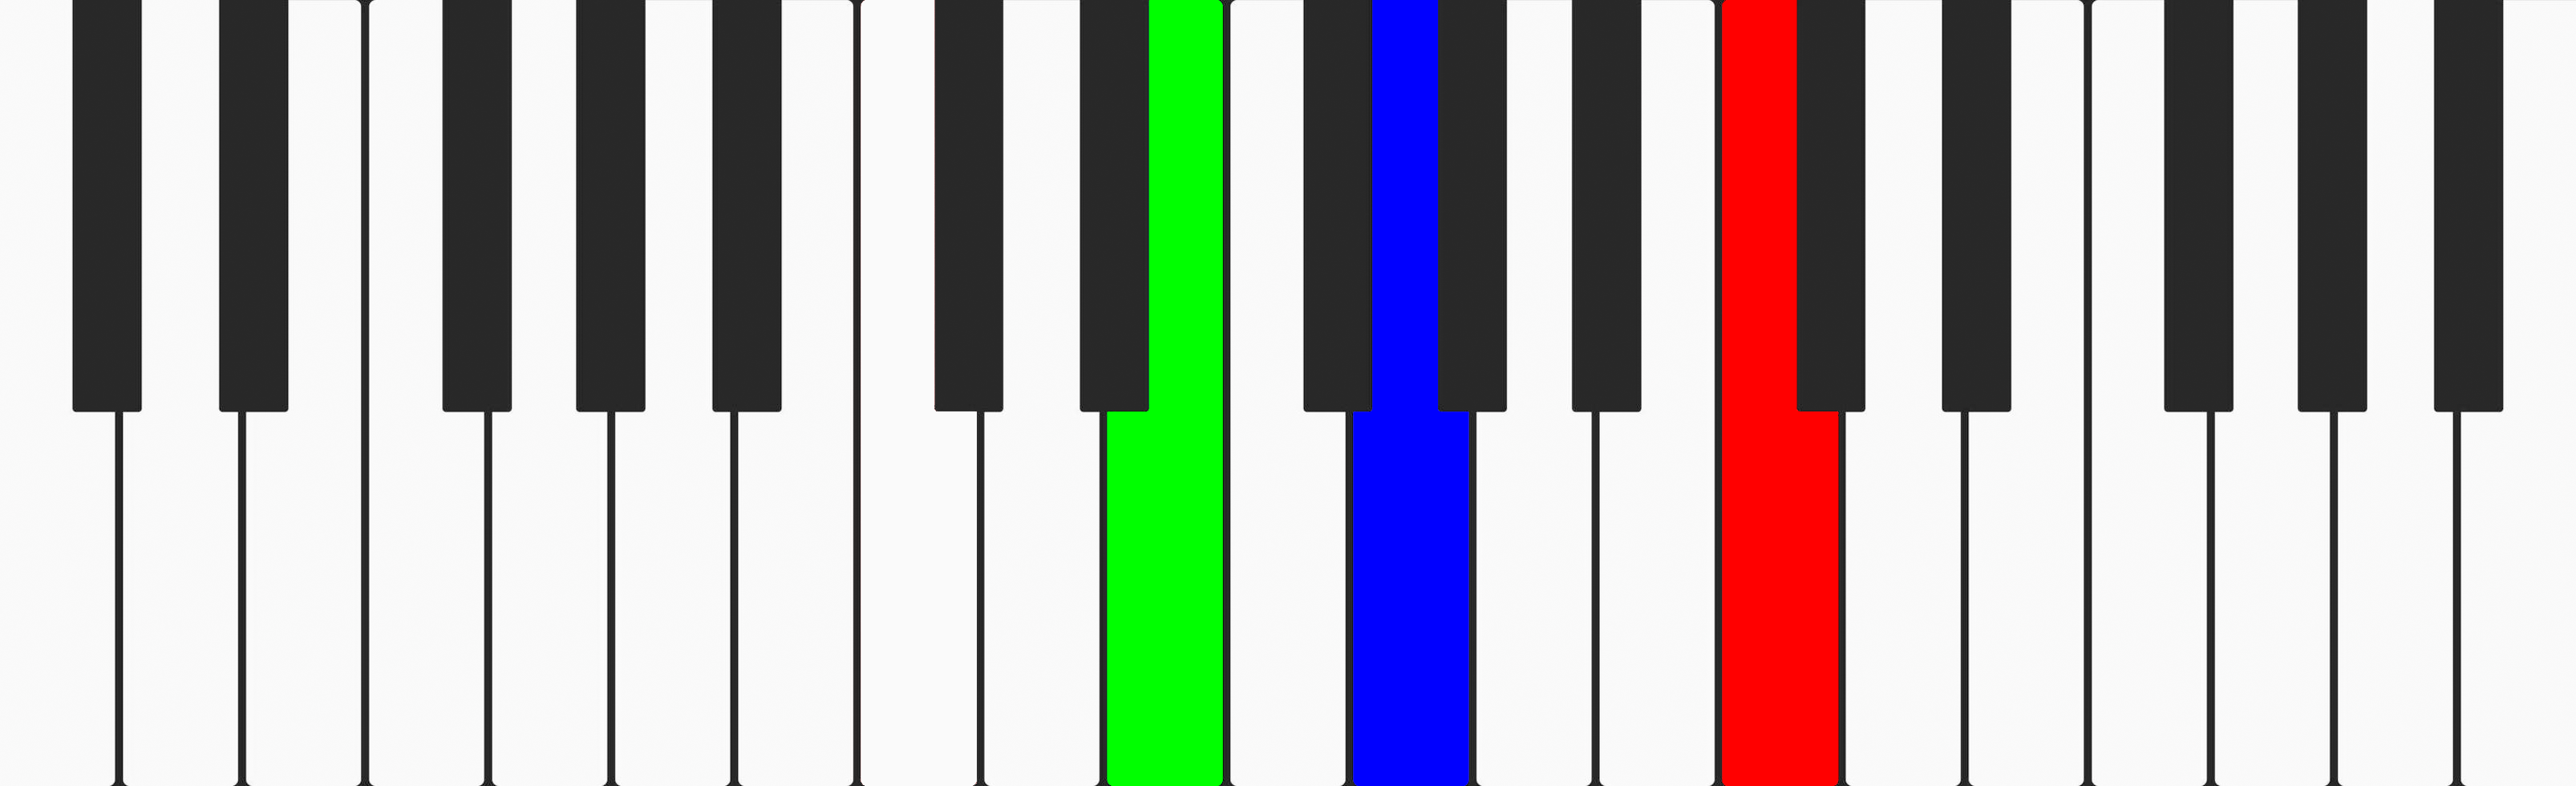
\includegraphics[width = 0.5\textwidth]{Imagenes/Bitmap/1era_inversion.png}
    \caption{Acorde de C en su 1ª inversión}
    \label{fig:inversion1}
\end{figure}

\begin{figure}[h]
    \centering
    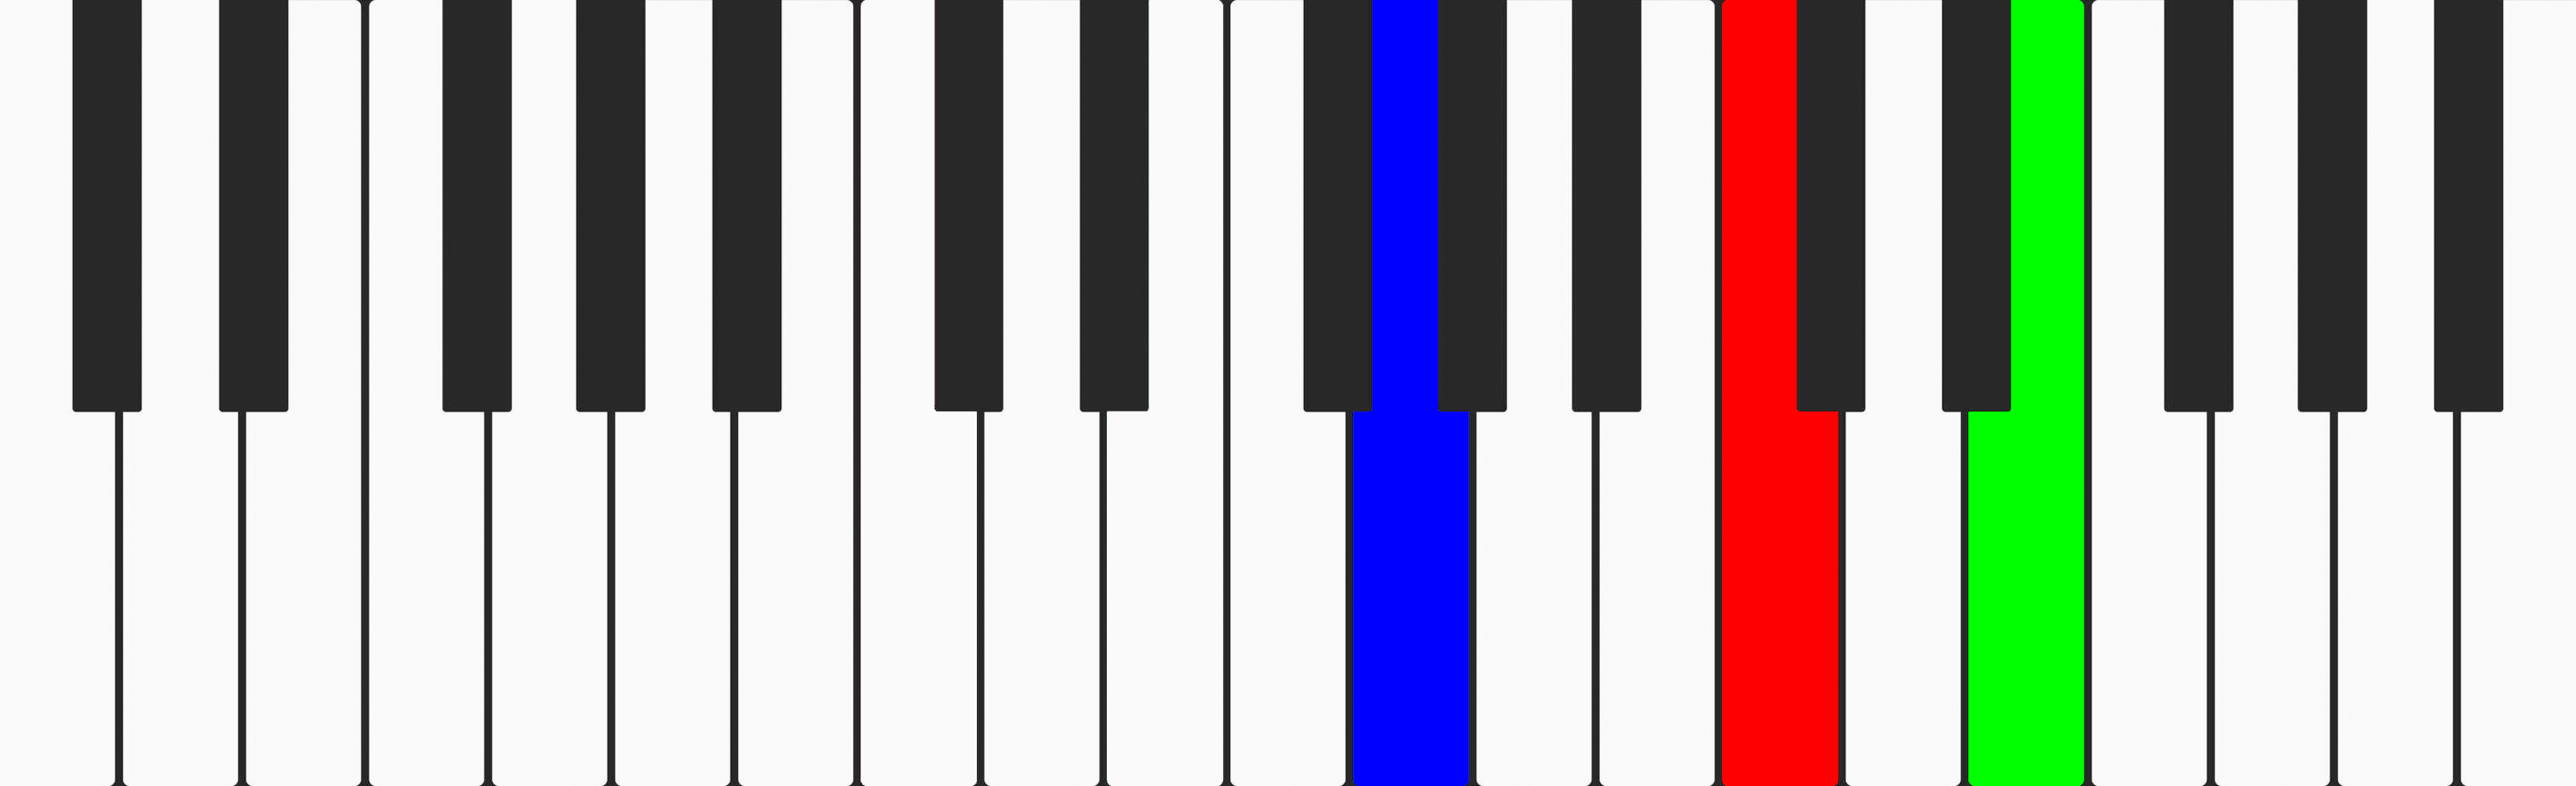
\includegraphics[width = 0.5\textwidth]{Imagenes/Bitmap/2da_inversion.png}
    \caption{Acorde de C en su 2ª inversión}
    \label{fig:inversion2}
\end{figure}

Esta no es la única forma en la que se puede encontrar un mismo acorde. Las notas que lo forman no tienen por qué ir consecutivas dentro de la misma octava o rango: (Figuras \ref{fig:inversion_extra1} y \ref{fig:inversion_extra2})

\begin{figure}[H]
    \centering
    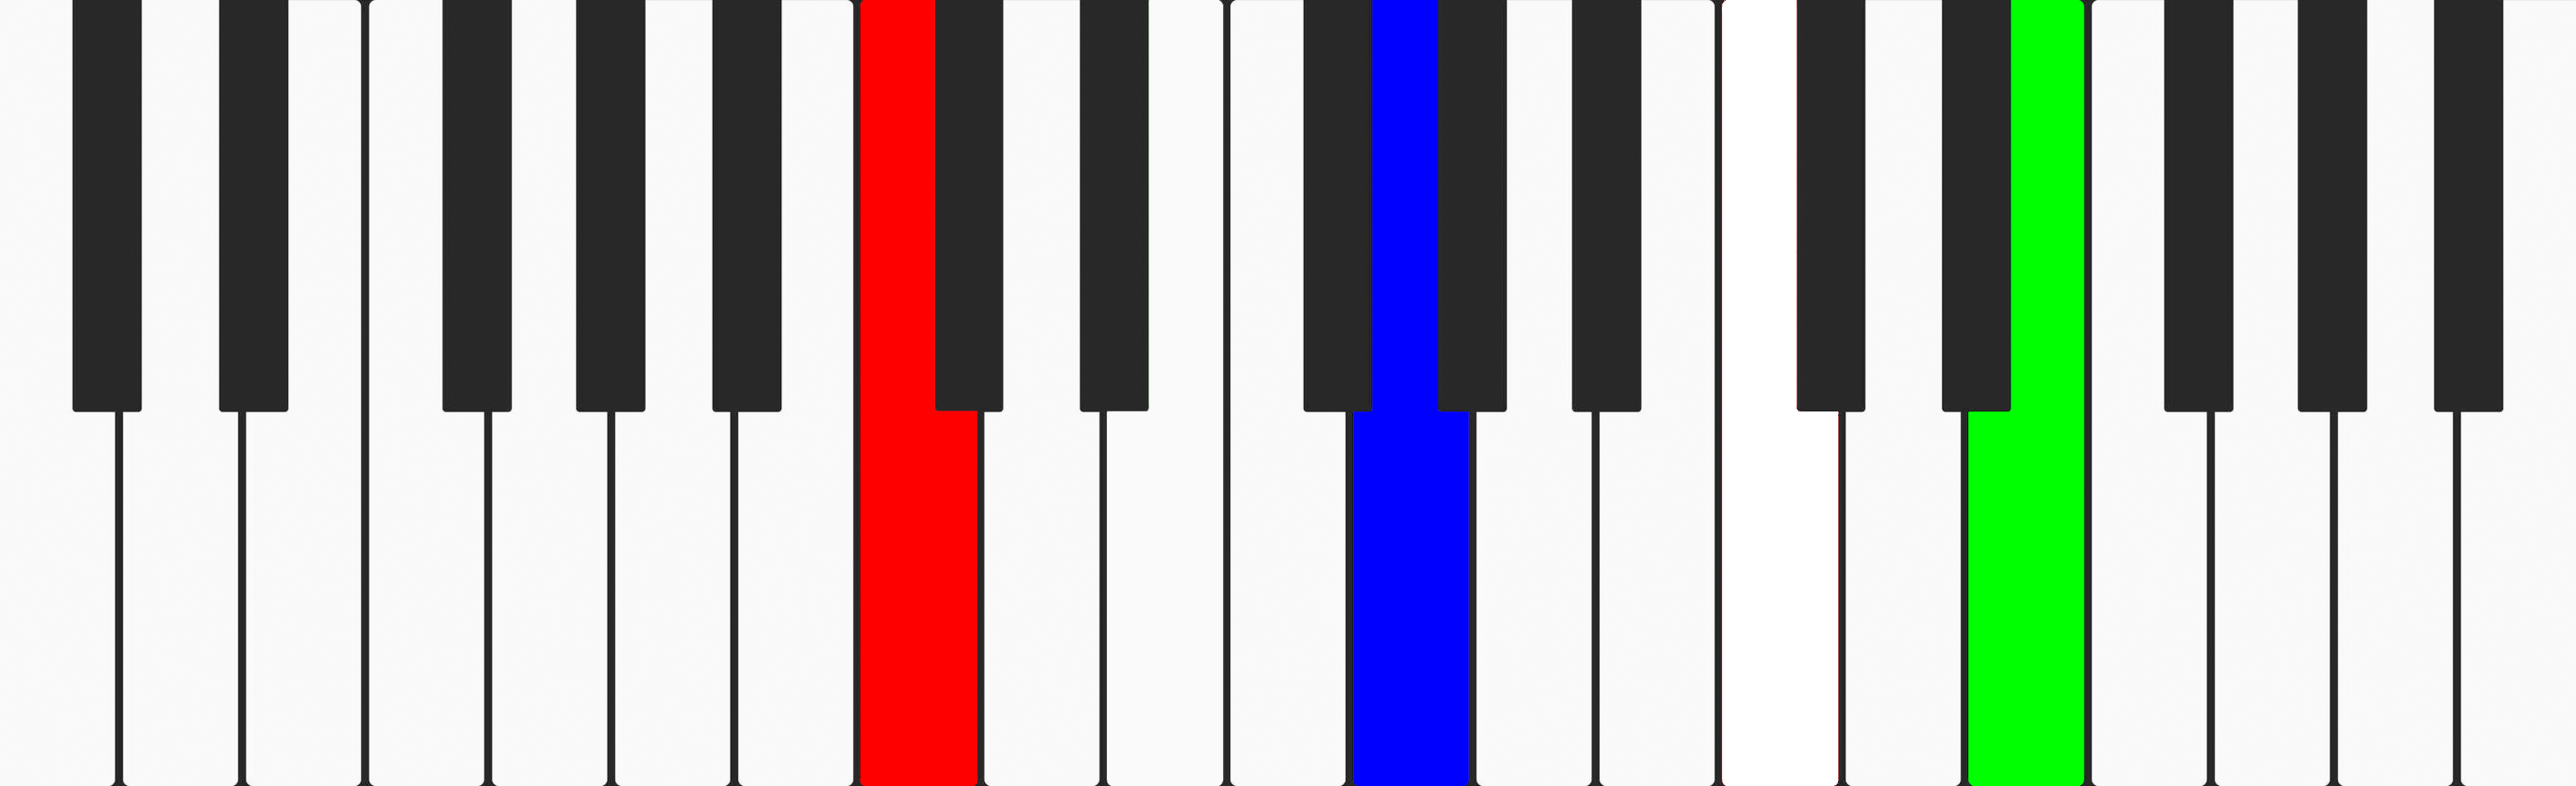
\includegraphics[width = 0.5\textwidth]{Imagenes/Bitmap/inversion_extra.png}
    \caption{Acorde de C en su estado fundamental con sus notas en diferentes octavas}
    \label{fig:inversion_extra1}
\end{figure}

\begin{figure}[H]
    \centering
    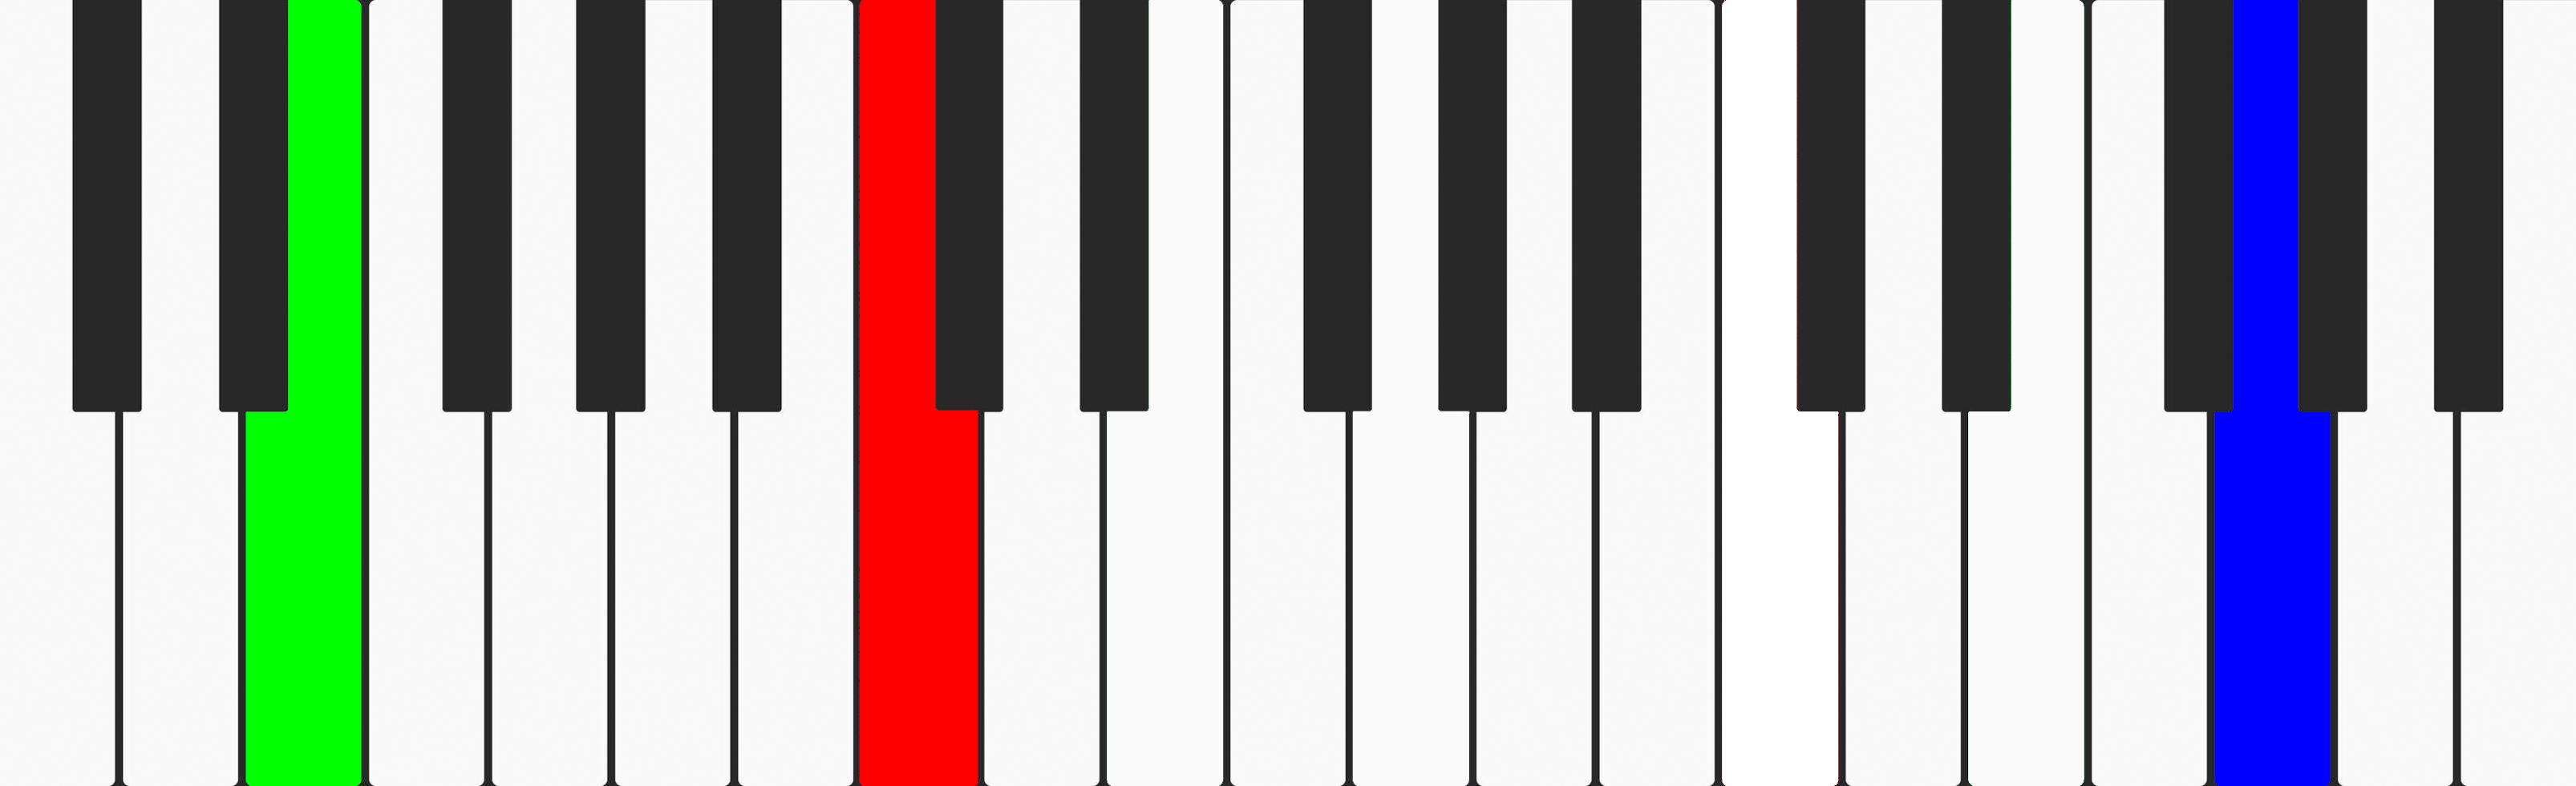
\includegraphics[width = 0.5\textwidth]{Imagenes/Bitmap/inversion_extra2.png}
    \caption{Acorde de C invertido con sus notas en diferentes octavas}
    \label{fig:inversion_extra2}
\end{figure}

Por supuesto, repetir notas del mismo acorde en diferentes octavas también se considera tocar dicho acorde: (Figura \ref{fig:inversion_extra3})

\begin{figure}[h]
    \centering
    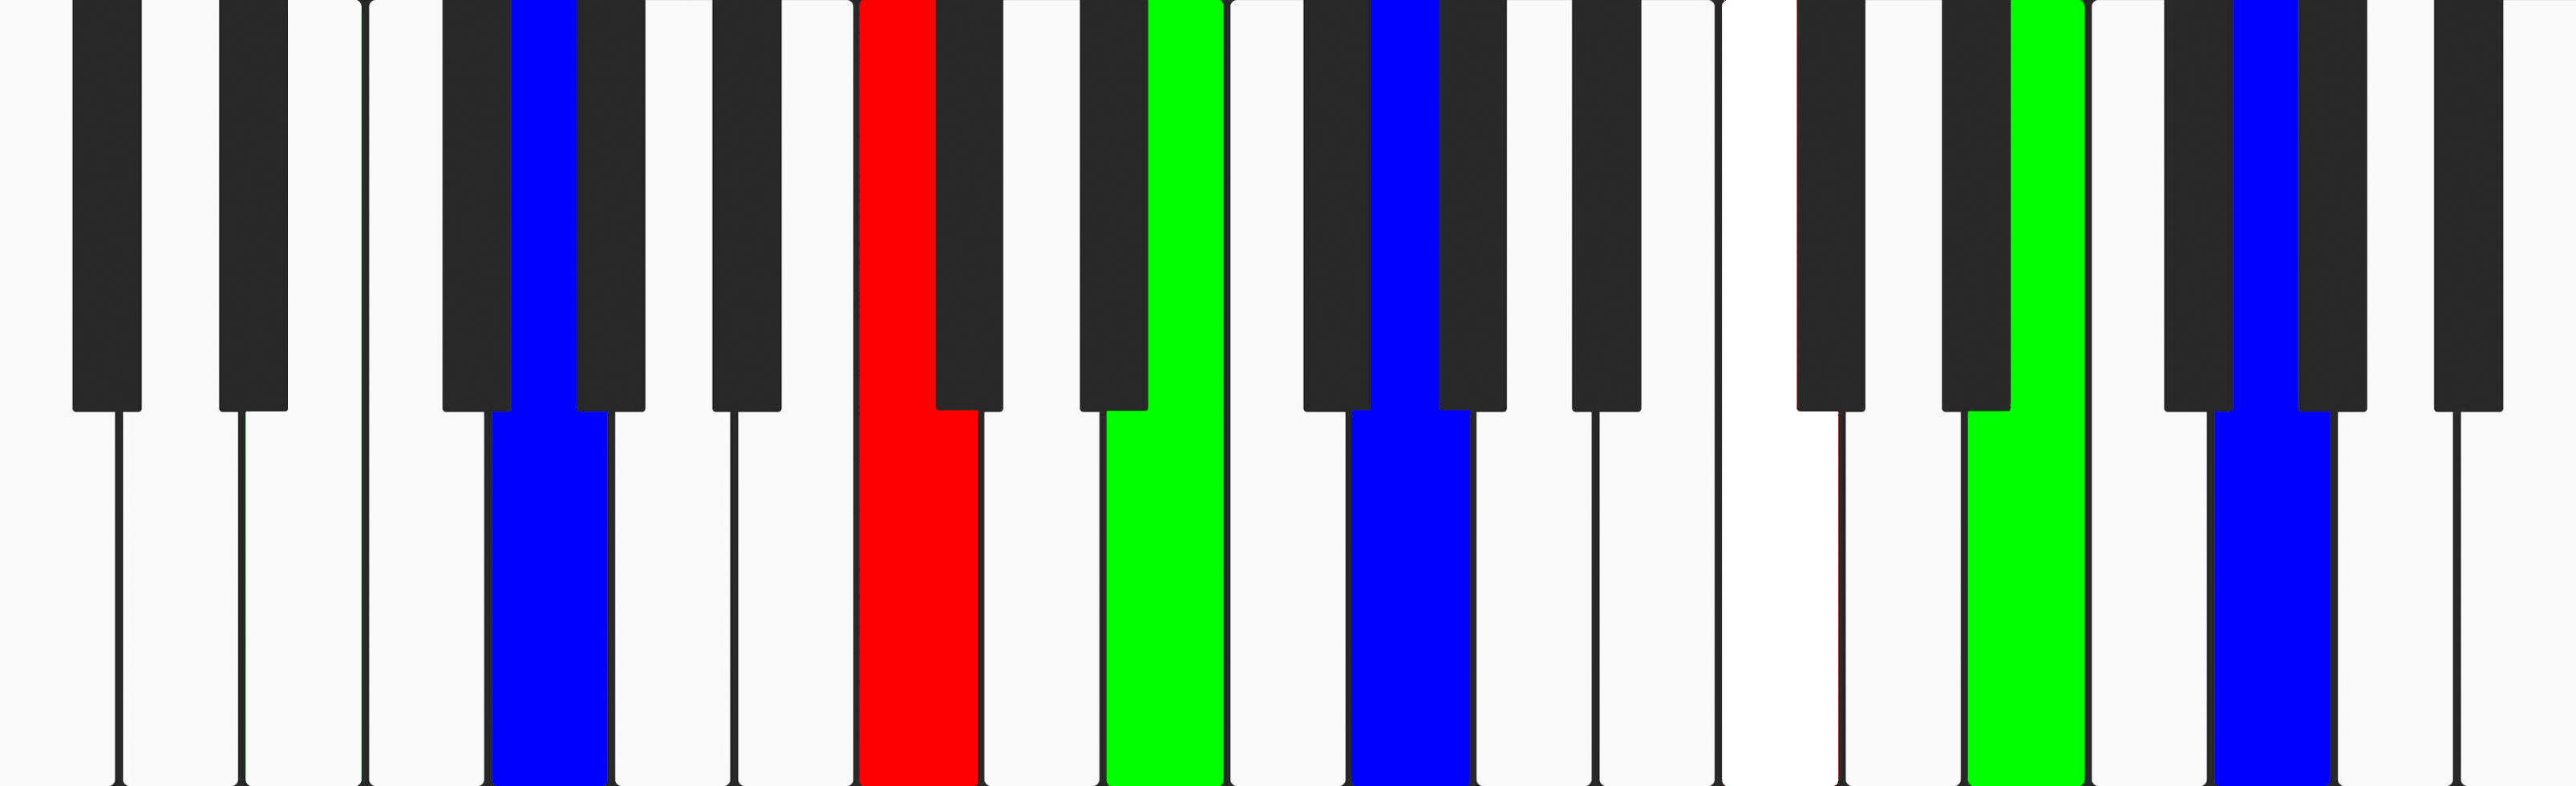
\includegraphics[width = 0.5\textwidth]{Imagenes/Bitmap/inversion_extra3.png}
    \caption{Acorde de C representado por múltiples notas}
    \label{fig:inversion_extra3}
\end{figure}

Con todos los ejemplos se quiere dejar claro que, a pesar de toda la combinatoria de representaciones que puede llegar a tener un mismo acorde y de las ligeras diferencias entre sus sonoridades, armónicamente simbolizan lo mismo, en este caso, el acorde de C.

\subsubsection{Arpegios}\label{subsec:arpegios}

Relacionado con las inversiones en el sentido de representar un mismo acorde pero de diferentes maneras, un arpegio se define como la secuencia de las notas del acorde tocadas de manera individual y sucesiva, pudiéndose encontrar estas en multitud de patrones diferentes. De nuevo, aunque la representación del acorde cambie, armónicamente simbolizaría lo mismo.

\subsection{Modos}\label{sec:modos}

Los modos de una escala son las diferentes secuencias de intervalos que se logran al comenzar una nueva escala desde los diferentes grados de la misma. La forma más sencilla de entenderlo es con un ejemplo en términos absolutos y relativizar cada escala obtenida pasándola a intervalos como se hace en la Tabla \ref{tab:modos_C} con la escala de C mayor (C jónico, en este contexto modal). Los modos de la escala mayor son los más utilizados, son los  conocidos como modos griegos, cada uno conocido con un nombre propio. A pesar de ello, este mismo proceso se puede realizar con cualquier escala.

\begin{table}[h]
    \centering
    \begin{tabular}{c|c|c|c|c|c|c|c|c|c|c|c|c|c}
        \multicolumn{1}{c}{}& \textbf{C} & D & E & F & G  & A & B & \textbf{C} & D & E & F & G & A\\
        \hline
        \hline
        \textbf{Jónico} & 1 & 2 & 3 & 4 & 5 & 6 & 7  \\
        \cline{0-8}
        \textbf{Dórico} & & 1 & 2 & b3 & 4 & 5 & 6 & b7 \\
        \cline{0-0}
        \cline{3-10}
        \textbf{Frigio} &\multicolumn{2}{c|}{} & 1 & b2 & b3 & 4 & 5 & b6 & b7 \\
        \cline{0-0}
        \cline{4-11}
        \textbf{Lidio} &\multicolumn{3}{c|}{} & 1 & 2 & 3 & \#4 & 5 & 6 & 7 \\
        \cline{0-0}
        \cline{5-12}
        \textbf{Mixolidio} &\multicolumn{4}{c|}{} & 1 & 2 & 3 & 4 & 5 & 6 & b7 \\
        \cline{0-0}
        \cline{6-13}
        \textbf{Eólico} &\multicolumn{5}{c|}{} & 1 & 2 & b3 & 4 & 5 & b6 & b7 \\
        \cline{0-0}
        \cline{7-14}
        \textbf{Locrio} &\multicolumn{6}{c|}{} & 1 & b2 & b3 & 4 & b5 & b6 & \multicolumn{1}{c|}{b7} \\      
        \cline{8-14}
    \end{tabular}
    \caption{Modos griegos}
    \label{tab:modos_C}
\end{table}

Viendo la tabla se pueden sacar varias conclusiones. La primera es que cada escala tiene tantas relativas con diferente tónica como modos tenga la propia escala. Aquí un ejemplo que sirve también para consolidar puntos descritos anteriormente: C jónico y D dórico son relativas entre sí porque comparten el mismo conjunto de notas, a pesar de tener distinta tónica; C jónico y C dórico no lo son porque aunque que comparten la misma tónica, el conjunto de notas que lo conforman es diferente, ya que el 'esqueleto' de sus escalas es diferente. La segunda conclusión es que el modo eólico es idéntico a la escala menor y que por lo tanto, en el caso del ejemplo, C mayor (jónico) es relativo a A menor (eólico). Hasta ahora se ha omitido, pero toda escala mayor tiene una relativa menor y viceversa.

Para consolidar aún más el concepto de los modos a continuación se van a mostrar varios ejemplos de modos griegos con tónicas diferentes a las descritas en la anterior tabla: (Tabla \ref{tab:otros_modos}

\begin{table}[H]
    \centering
    \begin{tabular}{c|c|c|c|c|c|c|c}       
        \textbf{Modo dórico} & 1 (T) & 2 & b3 & 4 & 5 & 6 & b7  \\
        \hline
        \textbf{C dórico} & C (T) & D & Eb & F & G & A & Bb  \\     
        \hline
        \hline
        \textbf{Modo lidio} & 1 (T) & 2 & 3 & \#4 & 5 & 6 & 7  \\
        \hline
        \textbf{A lidio} & A (T) & B & C\# & D\# & E & F\# & G\#    \\   
        \hline
        \hline
        \textbf{Modo locrio} & 1 (T) & b2 & b3 & 4 & b5 & b6 & b7  \\
        \hline
        \textbf{Eb locrio} & Eb (T) & Fb & Gb & Ab & Bb & Cb & Db  \\ 
    \end{tabular}
    \caption{Ejemplos de modos con distintas tónicas}
    \label{tab:otros_modos}
\end{table}

A pesar de no ser tan utilizados como las escalas mayor y menor, los modos y sobre todo, los modos griegos, son utilizados también en la música que solemos escuchar hoy por hoy. Difieren de sus relativas mayor y menor en el centro tonal. Como la tónica es distinta, los movimientos que surgen en una composición son distintos también, lográndose así colores nuevos. Aunque los modos formen parte de un capítulo más avanzado dentro de la teoría de la armonía, el conocimiento de su existencia y su origen son cruciales para el entendimiento de varios apartados del TFG.


\section{MIDI}
\label{subsec:que-es-midi}
A la hora de representar música, tradicionalmente hacemos uso una serie de estándares y normas que juntos forman la notación musical occidental. El uso de esta notación musical nos permite escribir partituras que otros músicos pueden entender e interpretar.

Pero, ¿cómo llevamos esto al mundo digital? Si bien hay programas capaces de interpretar partituras, en la mayoría de ocasiones se utilizan otras formas de lo que se denomina música simbólica. La más común es el MIDI (archivos con extensión .mid).

El MIDI, al igual que el resto de formatos de música simbólica, no suena por sí solo, pues el archivo no contiene sonido alguno. Al igual que una partitura, el MIDI nos indica qué nota hay que tocar, cuando hay que tocar esa nota, durante cuanto tiempo, y en ocasiones incluso en qué instrumento recomiendan ser tocadas esas notas (aunque esto último es algo que apenas se utiliza ya).

Como ya hemos dicho, el MIDI no contiene sonido, sólo instrucciones para tocar una serie de notas, por lo que es un formato de archivo muy liviano y cómodo de usar. Además, si bien podría parecer una desventaja no poder escuchar sin más su contenido, los sistemas operativos suelen traer una forma de reproducir el archivo MIDI fácilmente. En el caso de Windows, basta con abrirlo con el reproductor de multimedia por defecto para que lo interprete, eso sí, con timbres algo pobres pero que cumplen su función.

\section{Software musical}

\subsection{¿Qué es una DAW?}
Una DAW (Digital Audio Workstation) o estación de trabajo de audio digital, es un programa capaz de grabar y editar audio, producir, mezclar y masterizar música. También permiten  secuenciar música mediante MIDI y hacerla sonar mediante instrumentos virtuales.

Algunos ejemplos de DAWs populares son Ableton Live, Pro Tools, FL Studio o Reaper(Sección \ref{sec:reaper}), siendo esta última la que usaremos en nuestra herramienta.

\subsection{REAPER}\label{sec:reaper}
Reaper es la DAW que usaremos para generar sonido usando nuestra aplicación. Hemos escogido esta DAW por la facilidad que nos brinda para lanzar scripts sobre ella y por su precio, ya que cuenta con un periodo de prueba gratuito de 60 días con todas las funcionalidades del programa completo (sigue permitiendo su uso acabado el periodo de prueba). Además, el precio de Reaper es muy asequible comparado con el de otras DAWs.

En la Figura \ref{fig:captura-reaper} podemos ver la interfaz de Reaper. Hay tres pistas creadas, las dos primeras contienen algunos ítems MIDI y la tercera pista un archivo de audio que hemos cargado en formato .wav. Además, en la parte inferior de la interfaz se encuentra el mezclador o \textit{mixer}, donde podremos, entre otras cosas, regular el volumen de cada pista así como el de la mezcla resultante. También podemos desde este mezclador silenciar una pista (pulsando el botón con la letra M) o hacer que suene en solitario, silenciando el resto (pulsando el botón con la letra S).

\begin{figure}[h]
    \centering
    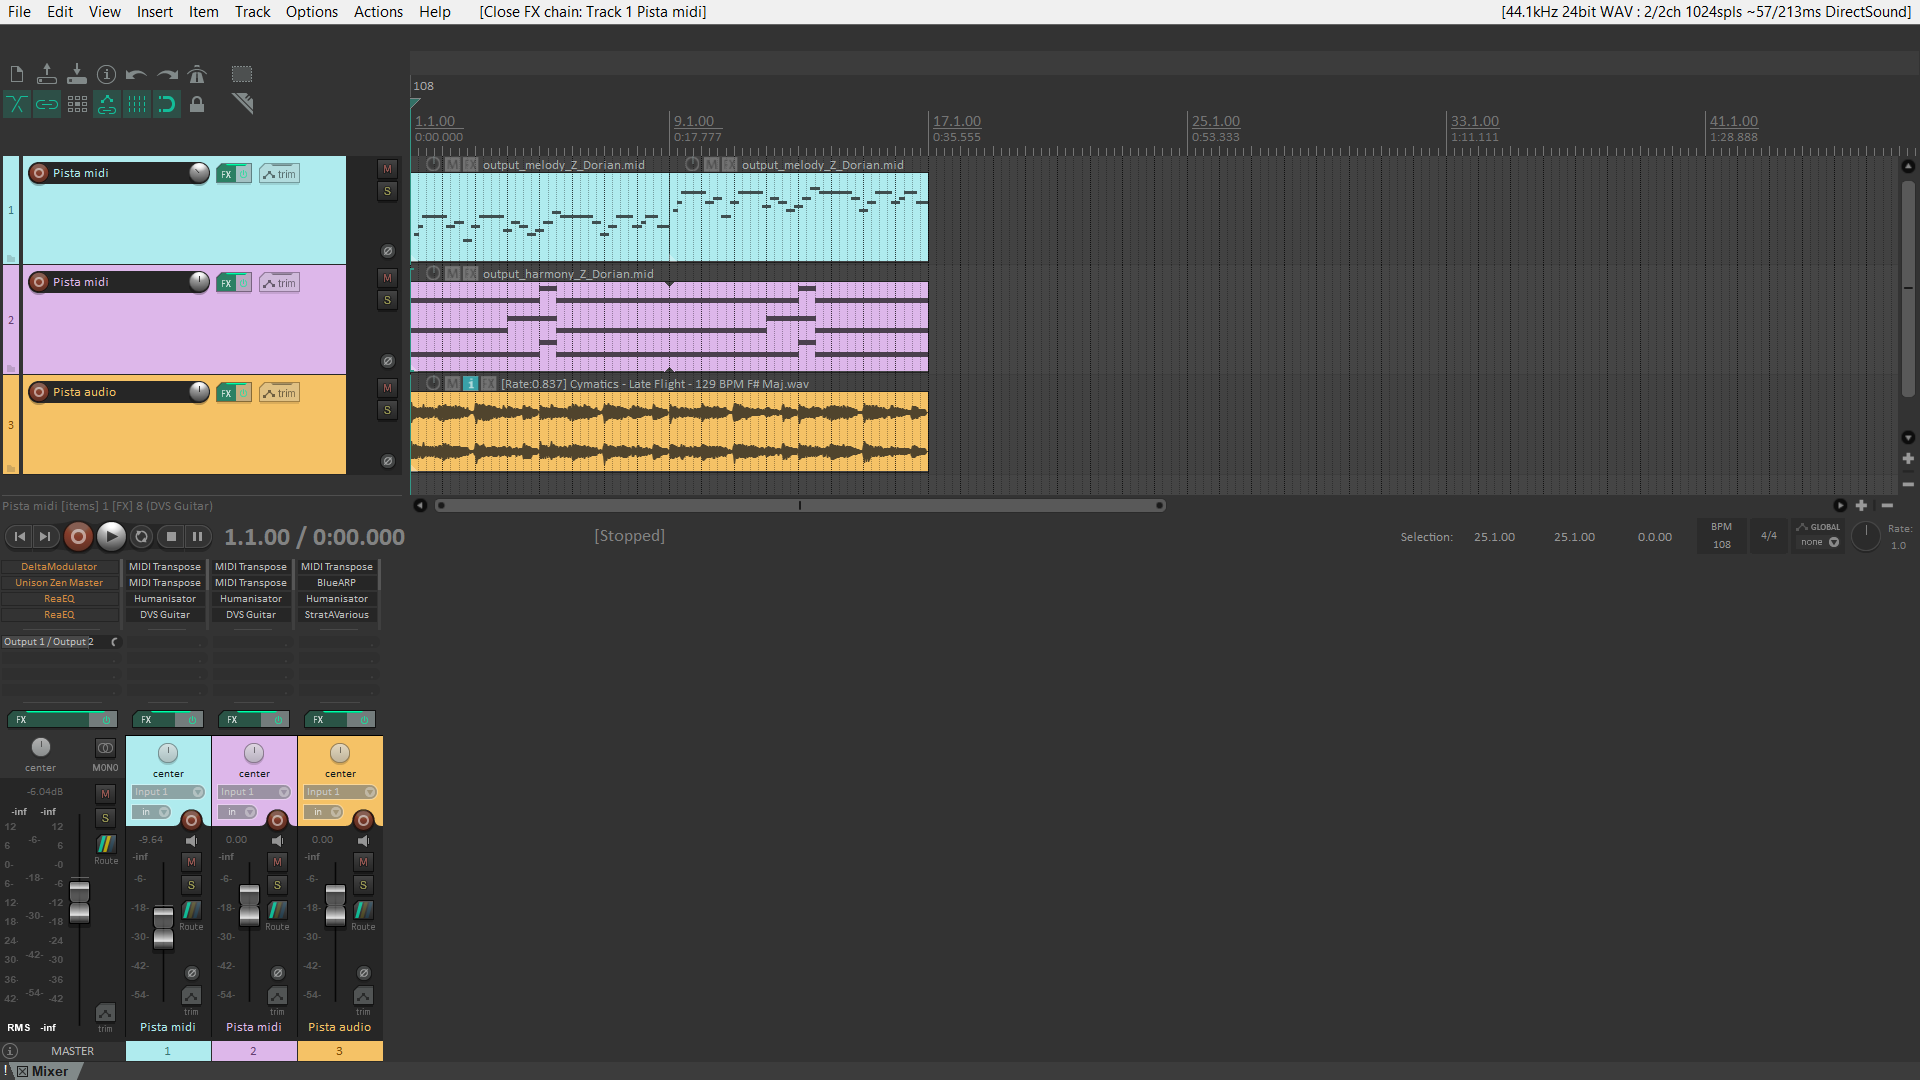
\includegraphics[width = 0.8\textwidth]{Imagenes/Bitmap/CapturaReaper.png}
    \caption{Captura de pantalla de Reaper}
    \label{fig:captura-reaper}
\end{figure}

Para preparar Reaper para trabajar con nuestra herramienta, consular el manual de usuario (Sección \ref{subsec:manual-reaper}).

\subsubsection{ReaScript}\label{subsec:reascripy}

Uno de los puntos fuertes de Reaper es su capacidad para ejecutar scripts, contando incluso con un editor de texto integrado donde podemos escribir scripts en Lua y Eel (un lenguaje de scripting propio de Reaper). Además de usando esos dos lenguajes, podemos llamar a las funciones de la API de ReaScript usando Python. Esta es la opción que hemos elegido por la comodidad que ofrece a la hora de programar.

Una vez escrito un script de Python (estando habilitado Python, ver su guía de uso en Sección \ref{subsec:manual-reaper}) podremos usar las acciones de Reaper para lanzar nuestro script. De forma alternativa, podemos lanzar el script sobre Python desde fuera, como lo hacemos desde la ventana de la herramienta (Sección \ref{sec:TK:app})

\subsection{Instrumentos}
Para poder generar audio usando una DAW, podemos reproducir sonidos muestreados o sintetizar sonidos en tiempo real. En una DAW, podemos escribir o cargar música simbólica, generalmente en formato MIDI (Sección \ref{subsec:que-es-midi}), en una pista. A continuación, podemos añadirle a esa pista un plugin de instrumento virtual, el cuál convertirá el MIDI en sonido.

Veamos un ejemplo: en la Figura \ref{fig:captura-reaper} se puede ver en la primera pista un ítem MIDI, abierto en el rodillo de piano en la Figura \ref{fig:rodillo-midi}. Dicho item generará una señal MIDI a medida que el cursor avance, señal que los plugins añadidos podrán modificar, y en el caso de los instrumentos virtuales (como el de la Figura \ref{fig:plugin-dvs}), convertir en audio.


\begin{figure}[h]
    \centering
    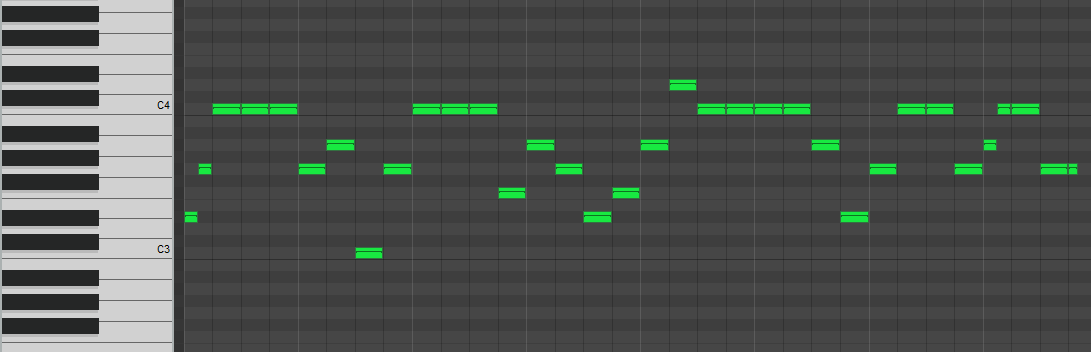
\includegraphics[width = 0.6\textwidth]{Imagenes/Bitmap/itemMidiAmpliado.png}
    \caption{Notas MIDI en el rodillo de piano de Reaper.}
    \label{fig:rodillo-midi}
\end{figure}

\begin{figure}[h]
    \centering
    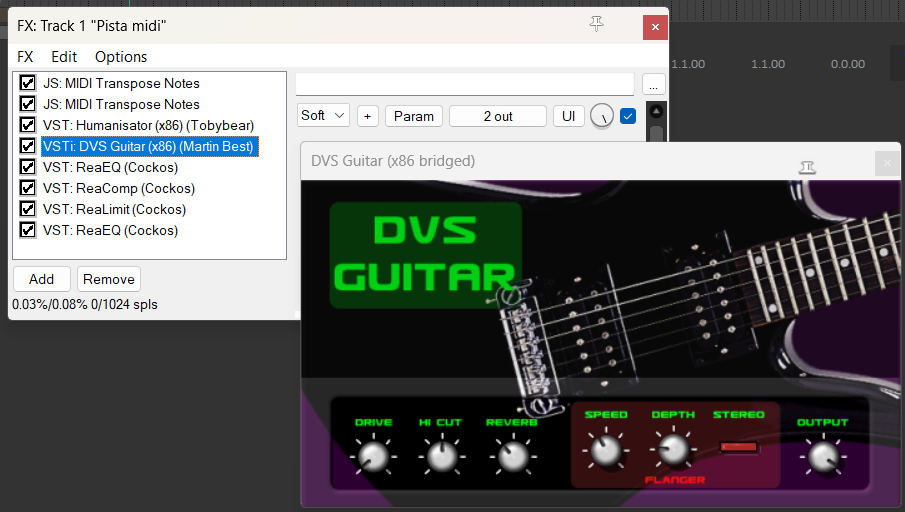
\includegraphics[width = 0.6\textwidth]{Imagenes/Bitmap/dvs.png}
    \caption{Un instrumento virtual de guitarra eléctrica, el DVS Guitar.}
    \label{fig:plugin-dvs}
\end{figure}


\subsubsection{¿Qué es un plugin?}\label{subsec:plugin}
Un plugin es un software externo (generalmente) que se carga en una DAW, en nuestro caso Reaper, para añadir distintas funcionalidades. En el ámbito de la producción musical, los plugins son fundamentales, ya que nos proporcionan instrumentos virtuales para generar sonidos y distintos efectos para manipular ese sonido.

El formato más común de los plugins en Windows son los VSTs (archivos con extensión .vst3 o .dll). Hay algunos otros formatos como AAX o AU, por ejemplo para dispositivos MAC, pero los que usaremos en nuestra herramienta son los mencionados VSTs. 

Podemos separar los plugins en varios tipos: Los efectos de audio, los plugins MIDI y los instrumentos virtuales.

Los efectos de audio reciben una señal de audio y la modifican de diversas formas. Algunos ejemplos de efectos de audio son la ecualización\footnote{\url{https://emastered.com/es/blog/equalizer-music}}, la reverberación (ver la Sección \ref{subsubsec:reverb}) o la compresión\footnote{\url{https://www.aulart.com/es/blog/que-es-la-compresion-y-como-usarla/}}.

Los plugins MIDI modifican una señal MIDI y la convierten en otra. Por ejemplo cambiando la octava de las notas, su intensidad, arpegiando dichas notas, etc.

Los instrumentos virtuales son plugins que transforman la señal MIDI en audio. Los instrumentos virtuales pueden separarse en varias categorías:
\begin{itemize}
    \item \textbf{Instrumentos sampleados}: Reproducen una muestra pregrabada al recibir un input MIDI. El número de muestras puede variar desde una muestra cada varias notas hasta decenas de muestras por nota, dependiendo de la intensidad de la nota (que en terminología MIDI es la "velocity"), o incluso varias muestras para una misma nota y misma intensidad (por ejemplo en un instrumento de percusión, golpeando en distintas zonas del tambor). Por tanto, para la mayoría de timbres ofrecen la mejor calidad de audio posible. Son instrumentos que suelen ocupar muchos gigabytes de almacenamiento, ya que las muestras en formatos de buena calidad (como el wav) ocupan mucha memoria.
    \item \textbf{Sintetizadores}: Crean sonido a mezclando distintas formas de onda, envolventes y efectos\footnote{\url{https://es.wikipedia.org/wiki/Sintetizador}}. Suelen usarse tradicionalmente en géneros de música más tirando a electrónica, pero hoy en día hay muchos usos para este tipo de instrumentos, ya que pueden usarse para recrear de forma más o menos realista la mayoría de timbres que podamos necesitar. Al no usar sonidos pregrabados, son alternativas más ligeras que los instrumentos sampleados.
    \item \textbf{Instrumentos mixtos}: Combinan muestras de sonidos o instrumentos reales con sonidos sintetizados en tiempo real.
\end{itemize}
